\chapter[Evaluation]{Evaluation}
\label{Chap:Evaluation}
% ***************************************************
%Evaluation 
% ***************************************************

\section{Raw Performance Benchmarks}
Here, the different configurations of VexRiscv: single-core, dual-core and quad core; will be compared in terms of performance alongside the Raspberry Pi Model 4B 1GB. For each one, we will run the performance benchmark, \textit{stress-ng}, which profiles the IO overhead and memory usage of multiple cores, along with \textit{Iperf3}, to gauge ethernet throughput capabilities.

\subsection{Iperf3}
As ethernet is a vital component of the application, it makes sense to evaluate the capabilities of the link, especially the average bitrate we can expect. After running \texttt{iperf3 -s}, which sets the device as a server and listens, another Raspberry Pi was chosen from the cluster to act as a client via running:
\begin{verbatim}    
iperf3 -c 192.168.1.50 -t 30 -i 1 -w 8K -P 1 -R
\end{verbatim}
This begins a single-threaded (\texttt{-P 1}), client that sends and receives TCP transmissions to \textit{192.168.1.50}, for 30 seconds, sampling the bitrate every second (\texttt{-i 1}). Most notably, it constrains the TCP window size (\texttt{-w 8K}), to 8Kb, which matches the current size of the board's TX or RX ethernet buffers, more closely resembling the stop-start transfers in our software setup. Here are the results:
\todo{Add reference to software/hardware overview}

\begin{table*}[ht]
    \centering
    \caption{Ethernet Throughput Comparison of Configurations}
    \begin{tabular}{lllll}
                                & \multicolumn{3}{l}{VexRiscvSMP, 100MHz} & RPi    \\ \cline{2-5} 
                                & Single        & Dual       & Quad       & 4B 1GB \\ \hline
    Amount Transferred (MB)     & 31.5          & 35.5       & 42.0       & 1.13k  \\
    Amount Recieved (MB)        & 31.4          & 35.4       & 41.9       & 1.13k  \\
    Sending Bitrate (MBits/s)   & 8.78          & 9.90       & 11.7       & 323    \\
    Receiving Bitrate (MBits/s) & 8.77          & 9.89       & 11.7       & 323    \\
    TCP Retransmissions         & 0             & 0          & 1          & 0      \\ \hline
    \end{tabular}
    \label{table:ethernet1}
\end{table*}

It is clear that the gigabit ethernet capabilities of the Raspberry Pi far outweigh the ethernet capabilities of the board, achieving 26x more throughput than that of the quad-core VexRiscvSMP. Keep in mind as well, the Raspberry Pi is throttled because of the 8Kb window size we set. Additionally, the core amount does have an effect on the bitrate as the quad core is 1.8MBits/s faster than the dual core, which is 1.12MBits/s faster than the single core. However, an overall improvement of 32\% across cores is basically negligible since the absolute performance is still far below what is required for what is essentially a high-speed ethernet application. It is clear from this benchmark alone that the bitrate will be a significant bottleneck for the design.

\subsection{Stress NG}
Stress-ng is a versatile benchmarking tool designed to stress test various components of a CPU. The command:
\begin{verbatim}
stress-ng --cpu $CORE_COUNT --io 2 --vm 1 --vm-bytes 128M --timeout 60s 
--metrics-brief
\end{verbatim}
Runs a set of tests in parallel. The rest of the arguments determine the amount of tests and the type: \texttt{--cpu}, creates CPU-intensive tasks equal to the core count; \texttt{--io}, creates two I/O-intensive tasks; and \texttt{--vm}, allocates and uses 128MB of virtual memory. This will evaluate for us how the system performs under combined CPU, I/O, and memory pressure, as well as how these metrics vary with the amount of cores. Additionally, the test will timeout after 60 seconds or until $6\cdot$\texttt{\$CORE\_COUNT} CPU bogo ops have been completed. Here are the results:

\begin{table*}[ht]
    \centering
    \caption{Stress-ng Comparison of Configurations}
    \begin{tabular}{lllll}
                                  & \multicolumn{3}{l}{VexRiscvSMP, 100MHz} & RPi       \\ \cline{2-5} 
                                  & Single      & Dual        & Quad        & 4B 1GB    \\ \hline
    CPU bogo ops                  & 6           & 12          & 24          & 12,483    \\ \hline
    CPU real time (s)             & 125.34      & 119.09      & 121.30      & 60.03     \\
    CPU usr time (s)              & 78.32       & 164.00      & 378.16      & 146.85    \\
    CPU sys time (s)              & 0.01        & 0.12        & 0.09        & 0.03      \\
    CPU bogo ops/s (real time)    & 0.05        & 0.10        & 0.20        & 207.94    \\
    CPU bogo ops/s (usr+sys time) & 0.08        & 0.07        & 0.06        & 84.99     \\ \hline
    IO bogo ops                   & 21,794      & 31,190      & 27,819      & 440,066   \\ \hline
    IO real time (s)              & 60.00       & 60.01       & 60.00       & 60.00     \\
    IO usr time (s)               & 2.74        & 3.56        & 3.42        & 10.34     \\
    IO sys time (s)               & 25.71       & 44.44       & 66.44       & 48.56     \\
    IO bogo ops/s (real time)     & 363.22      & 519.76      & 463.65      & 7,334.31  \\
    IO bogo ops/s (usr+sys time)  & 766.05      & 649.79      & 398.21      & 7,472.11  \\ \hline
    VM bogo ops                   & 2,280       & 3,053       & 2,464       & 617,668   \\ \hline
    VM real time (s)              & 61.92       & 62.54       & 61.54       & 60.16     \\
    VM usr time (s)               & 7.57        & 10.72       & 18.10       & 27.27     \\
    VM sys time (s)               & 7.60        & 14.93       & 18.32       & 6.78      \\
    VM bogo ops/s (real time)     & 36.82       & 48.82       & 40.04       & 10,266.29 \\
    VM bogo ops/s (usr+sys time)  & 150.30      & 119.03      & 67.66       & 18,143.58 \\ \hline
    Total time taken (s)          & 125.45      & 120.31      & 122.76      & 60.00     \\ \hline
    \end{tabular}
    \label{table:stress1}
\end{table*}
\raggedbottom

\begin{figure*}[ht]
    \centering
    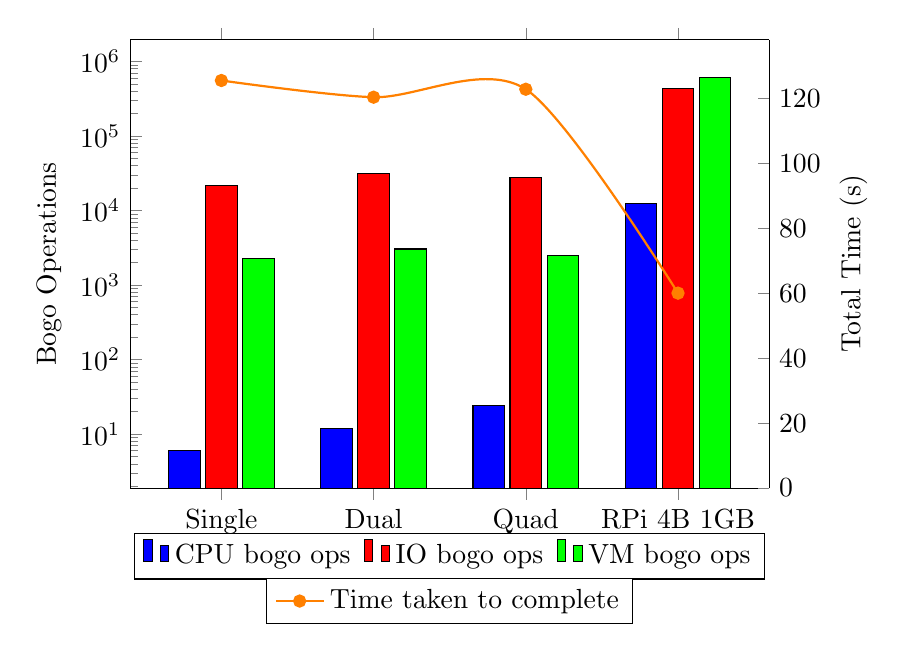
\begin{tikzpicture}
    \begin{axis}[
        width=0.8\textwidth,
        height=0.6\textwidth,
        ybar,
        bar width=0.4cm,
        enlarge x limits=0.2,
        legend style={
            at={(0.5, -0.1)},
            anchor=north,
            legend columns=-1,
            /tikz/every even column/.append style={column sep=0.1cm}
        },
        ylabel={Bogo Operations},
        symbolic x coords={Single, Dual, Quad, RPi 4B 1GB},
        xtick=data,
        axis y line*=left,
        ylabel near ticks,
        ymode=log,
        log origin=infty,
        ]
    \addplot[fill=blue] coordinates {
        (Single,6) (Dual,12) (Quad,24) (RPi 4B 1GB,12483)};
    \addplot[fill=red] coordinates {
        (Single,21794) (Dual,31190) (Quad,27819) (RPi 4B 1GB,440066)};
    \addplot[fill=green] coordinates {
        (Single,2280) (Dual,3053) (Quad,2464) (RPi 4B 1GB,617668)};
    \addlegendentry{CPU bogo ops}
    \addlegendentry{IO bogo ops}
    \addlegendentry{VM bogo ops}
    \end{axis}
    
    \begin{axis}[
        width=0.8\textwidth,
        height=0.6\textwidth,
        enlarge x limits=0.2,
        legend style={
            at={(0.5,-0.2)},
            anchor=north,
            legend columns=-1,
            /tikz/every even column/.append style={column sep=0.5cm}
        },
        axis y line*=right,
        axis x line=none,
        ylabel={Total Time (s)},
        ylabel near ticks,
        ymin=0,
        symbolic x coords={Single, Dual, Quad, RPi 4B 1GB},
        ]
    \addplot[smooth, thick, orange, mark=*] coordinates {
        (Single,125.45) (Dual,120.31) (Quad,122.76) (RPi 4B 1GB,60.00)};
    \addlegendentry{Time taken to complete}
    \end{axis}
    \end{tikzpicture}
    \caption{Stress-ng Performance Comparison Across Configurations}
    \label{fig:stress2}
\end{figure*}

Immediately, we are presented with an extreme difference in performance scaling, which is to be expected when comparing an FPGA-based softcore processor to a Raspberry-Pi single-board computer. There is still nuance, however, between the different core configurations of the VexRiscvSMP. For instance, the amount of CPU bogo ops tend to scale linearly with the core count, maintaining a similar execution time (see "CPU real-time" in table: \ref{table:stress1}). Other than this, there are no clear trends for the IO or VM bogo operations. It seems that once we extend to four cores, there are resource contentions with the IO bus and memory, leading to the quad core performing slightly less favourably than the dual core in these operations. Therefore, IO and memory have the potential to be another two bottlenecks, in addition to the low ethernet throughput, (although ethernet is still the dominant bottleneck). This can give us an estimation of how the dual core will perform relative to the quad core, \ie, it may end up performing better since the quad core will not only have to contend with IO/memory constraints from the shared DRAM\todo{make reference to hardware overview}, but also the limited ethernet buffers.

Overall, out of the VexRiscvSMPs, dual core performed the best, but only if we exclude raw CPU power. As our application depends more on resource read/writes and management, dual core may prove to be the best configuration; besides the Raspberry Pi of course.
\raggedbottom

\section{Results \& Analysis}
In this section, we will now compare how each configuration performed running the exact same full suite of tests on our application\todo{Make reference to software setup}. We will then take the best performing out of the VexRiscv configurations and see if we can improve the design to achieve even more throughput.

\subsection{Test Suite Full Outline}
The tests will focus only on encryption, since decryption and encryption times are the same, and we have proven that the device is encrypting properly\todo{add reference to proof of encryption}. We are aiming to deduce how each configuration performs with single or multiple clients. Therefore, the test outline is as such:
\begin{enumerate}
    \item Basic test 1: \\
    1 client with 1 100mb file.
    \item Basic test 2: \\
    10 clients with varying file sizes.
    \item Basic test 3: \\
    20 clients with varying file sizes, in 10 client chunks
    \item Large scale test: \\
    100 clients with varying files sizes, in 10 client chunks
\end{enumerate}


While these tests are running, we are collecting a multitude of metrics regarding overall performance\todo{Make reference to database}, but the primary result we are concerned with is the total bytes processed (or bytes encrypted) per second. This single metric is fundamentally all we need to determine which amount of cores is superior.
\subsection{Single Core Results}

% \begin{figure}[h]
%     \begin{center}
%     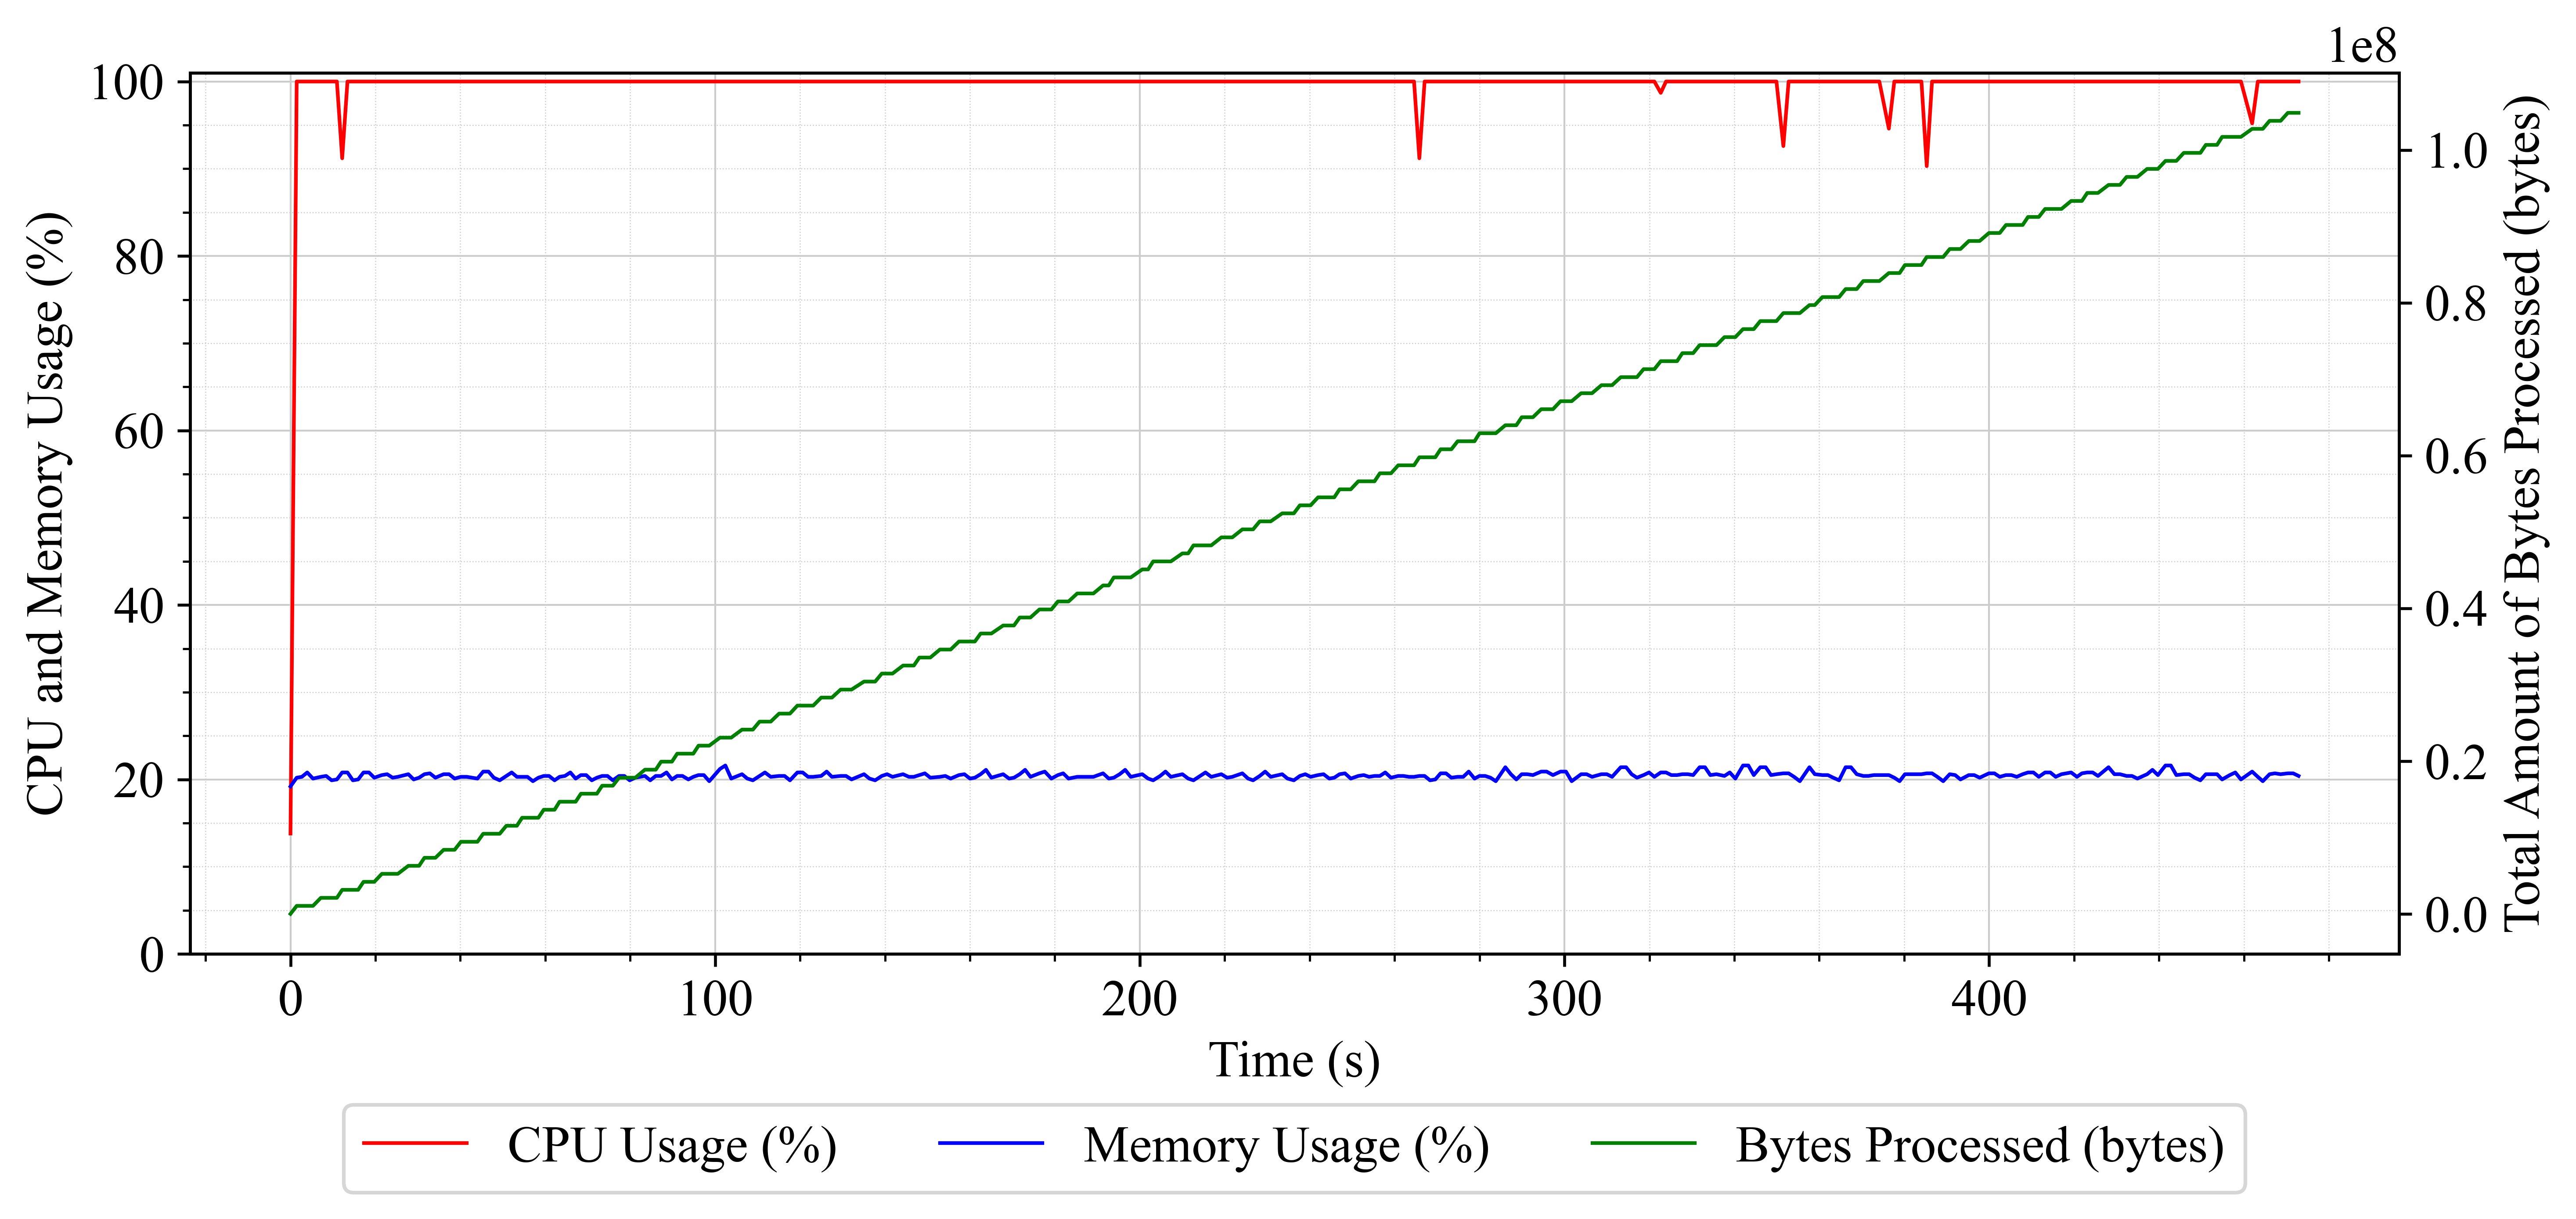
\includegraphics[width=1.0\textwidth]{Chapter4/Results/1c_results/arty-a7-1c_basic_1_20241004_110917.db_server_metrics.png}
%     \caption{The University Of Queensland}
%     \label{Fig:1}
%     \end{center}
% \end{figure}


\subsection{Dual Core Results}
\subsection{Quad Core Results}
\subsection{Raspberry Pi Results}
\section{Improved Dual-Core Design, Results and Analysis}
\section{Utilisation, Resources and Timing}
\section{Power Usage}